\documentclass[12pt]{article}
\usepackage{graphicx}
\usepackage{titlesec}
\usepackage{xlop}
\usepackage{url}
\usepackage{subcaption}
\usepackage{geometry}
\graphicspath{ {./images/} }
\usepackage[fleqn]{amsmath}
\usepackage{tikz}
\usepackage{listings}
\usepackage{karnaugh-map}
\geometry{
    a4paper, 
    top=20mm,
    left=20mm,
}
\setlength{\parindent}{4em}
\setlength{\parskip}{1em}
\renewcommand{\baselinestretch}{1.5}

\title{Final Project: ES4 Spring 2021}
\date{5/11/2021}
\author{Ibrahima Barry, WIlly Lin \\ Zach Osman, James Eidson \\ ECE Tufts University}

\titleformat{\section}
    {\normalfont\Large\bfseries}{\thesection}{1em}{}[{\titlerule[1pt]}]

\lstdefinestyle{myListingStyle} 
    {
        basicstyle = \small\ttfamily,
        breaklines = true,
    }

\begin{document}

\maketitle

\begin{flushleft}

\section{Overview}
\begin{center}
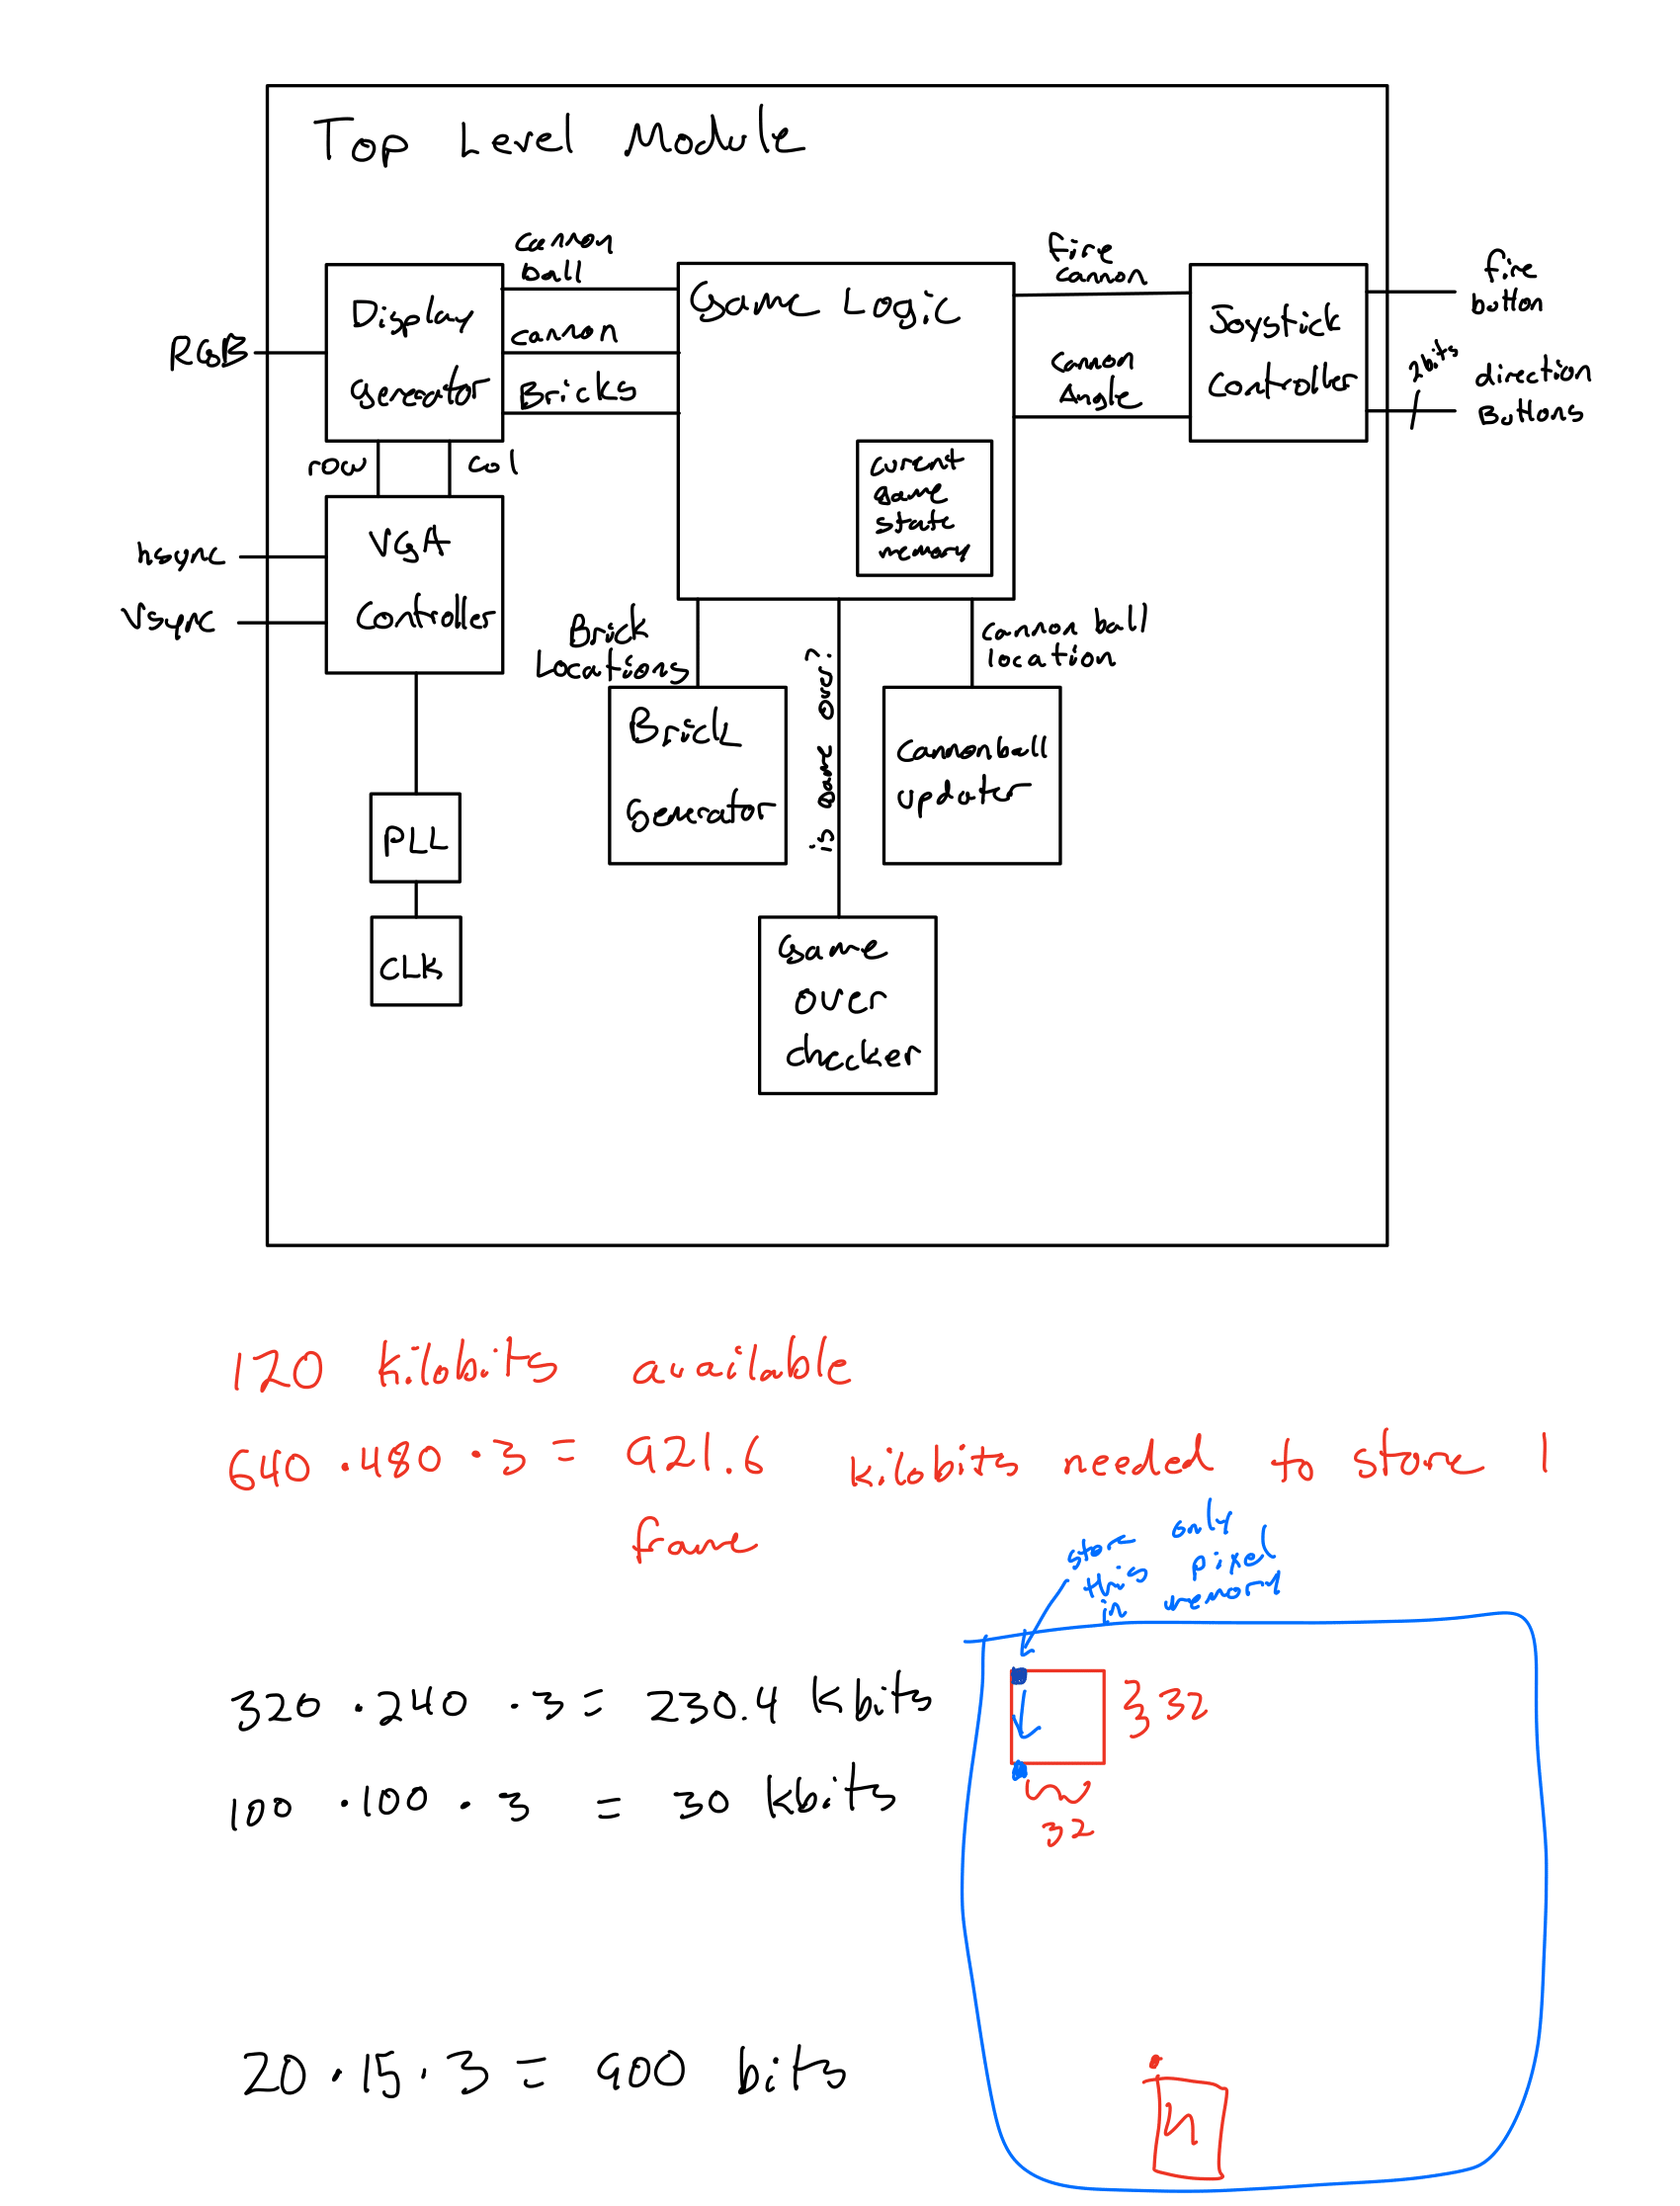
\includegraphics[width=10cm, height=10cm]{blockDiagram}
\end{center}
This game is a variation of the game brickBreaker where the player fires a
cannonball out of a cannon and works to destroy the bricks that are displayed on
the screen. There are three main parts to this project: displays, controls, and
game logic. 'Displays' were done using a VGA, 'controls' were done by using
an NES gamepad, and 'game logic' done in the 'top' module of our project. 
VGA sends the current row and column to display on the screen. The NES gamepad
takes data in the form of buttons pressed and stores it in a shift-register. A
clock is driven for 8 cycles (the number of buttons is 8) and the data signal is
synchronized with the clock. When a button is pressed the corresponding bit of
the output of the register is set to low. The top module controls the general
logic of the game such as drawing the bricks and the cannnon. Top also controls
the memory usage of the game. Overall, objects are drawn in the top module,
displayed via the display module, and those objects are then controlled via the
cannon module (which is connected to the gamepad). 

\section{Technical Description and Design}
\subsection{Top Module}

The top module is where the main game logic is handled. It's inputs are the
12MHz clock of the FPGA and the data from the the controller. It outputs the
necessary signals for the controller and the VGA to work. It's components
are the pll, vga, display, and cannon. The main function of top is to draw the
game objects. This the code to draw the bricks:\\
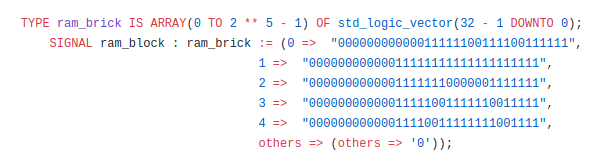
\includegraphics[width=15cm, height=5cm]{drawingBricks}

Where there is a '1' bit is where a brick is drawn. The other details are more
complicated but in general $'1' = $ brick drawn $'0'=$ brick not drawn. $0 - 4$
represent the row being drawin. One of the major challenges encountered here was
figuring out how to destroy a brick when it is hit by a cannon. This means where
there is a $'1'$ bit, meaning a block is drawn at that position, we have to invert
the bit when it is hit by the ball. The display module now knows not to draw
that brick. This was solved by using bit-masking to change the bit.\\ 
eg) consider the row of bricks: $00000000000011111100111100111111$
suppose the block at index 31 needs to be destroyed then the $XOR$ logical
operation works well for this. 
$00000000000011111100111100111111 \oplus 00000000000000000000000000000010 =
00000000000011111100111100111101$ 

We create a new bit word of the same size as the ram block  with the corresponding bit we want destroyed to be '1'
and the other bits to '0'. Then $ 1 \oplus 1 = 0$ so this will invert the bit we
want inverted. The other bits are unchanged as $1 \oplus 0 = 1$ and $0 \oplus 0 = 0$.  
A schematic of our top module is shown below:\\
\begin{center}
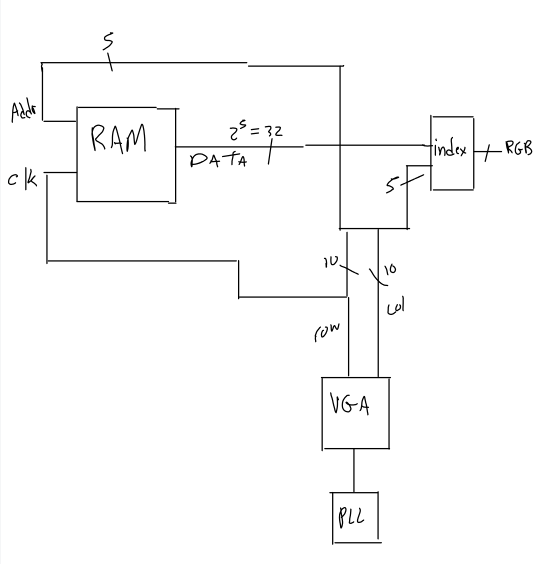
\includegraphics[width=10cm, height=10cm]{displayDiagram}
\end{center}
\subsection{Display Module}
The VGA module is responsible for sending the current row and column that we are
writing to the display. It outputs the HSYNC and VSYNC as well as the 10-bit
unsigned for the row and column number.\\ 
\hfill \break
The display module is responsible for setting the rgb value of pixels on the
screen. This module takes in the row and column we are writing to from the VGA,
as well as the position of the cannon, cannonball, and bricks. Using a process
block, we color pixels whose row and column match the positions of the cannon,
cannonball, or bricks. Since the bricks are only represented as a single bit in
RAM, our condition for coloring the pixels colors a 32 x 32 pixel area based on
the single bit provided by the RAM.

\subsection{Cannon Control Module}
\begin{center}
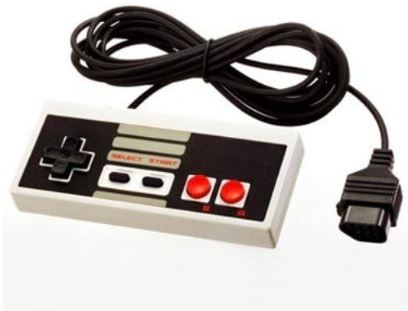
\includegraphics[width=8cm, height=8cm]{nes}
\end{center}
This is where the NES gamepad is used to control our game objects: the cannon
and the cannon ball. Cannon sends it's data signal (which is also in the top
module) to the NES controller and outputs the ball and cannon position based on
the which button is pressed. Instead of using all 8 bits of the output of the
NES only three were used the left and right button to move the cannon
horizontally and the "A" button to fire the cannon ball. The rest of the bits
were sent to 0. \\
\hfill \break
The logic for moving the cannon was relatively simple: if the button is pressed
(the signal is low) change the cannon's position by 1 to the left or right (which is later used in the top
and display modules in order to actually display the change). If the fire button
is pressed: change the row the ball is displayed (move the ball up) else set the
column of the ball to the cannon's colum and it's row to the cannon's row as
well. \\

\hfill \break
The biggest challenge we had was figuring out how to smoothly fire the cannon
ball. The firing was happening too rapidly, pressing the button jumped the ball
too far up the screen. The solution we came up with was to have the ball
continously be where the cannonis and if the user presses the fire button the
ball goes up and stops once the user stops pressing the button. THe ball shot
4-24 times based on how long the button was held. 
\section{Results and Testing}

Overall, we were able to create a functioning game that is able to be controlled
using the vga controller. It is able to move left and right and shoot the bricks
and delete or destroy them in the process if the position of the cannonball is
the same as the bricks. There were a few parts of our project we were not able
to implement. We were not able to make the bricks different colors and change
the angle of shooting. We were also not able store “levels” so randomly
generated bricks to be added in every few seconds to make the game harder.
Moreover we were missing a game over functionality. If we had more time, we
would like to add all of these things. 

This is the initial state of the game: \\
\begin{center}
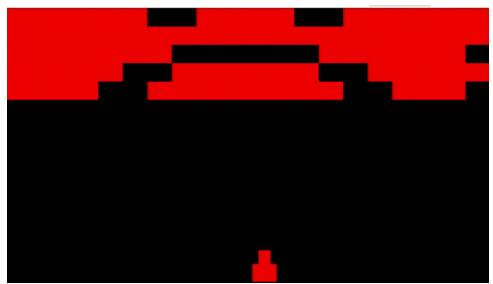
\includegraphics[width=10cm, height=8cm]{game1}
\end{center}

After firing some cannon balls some of the bricks were destroyed and this is
ther result:\\
\begin{center}
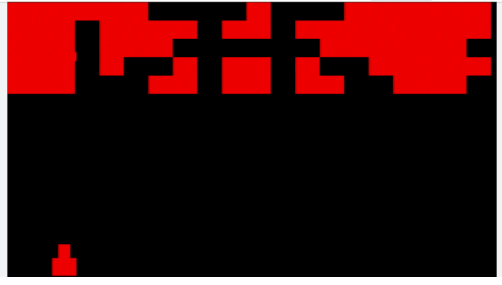
\includegraphics[width=10cm, height=8cm]{game2}
\end{center}

The game did have some bugs at the end however:\\
\begin{enumerate}
    \item The cannonball does not move smoothly and can only move if the fire
button is held. It also doesn’t go through each row and skips rows so it might
not destroy all the blocks at once. 
    \item Sometimes the connection isn’t tight or fully connected so it would randomly move or shoot.
    \item The firing is not exactly very smooth and might skip some bricks that
were supposed to be deleted.
\end{enumerate}

\section{Reflection} 
This project overall was fairly difficult and a lot of issues occurred. I think
next time we should have planned the modules, especially the brick diagram more
closely and specifically so it would be easier to implement the vhdl. In
addition if we can add anything it would add complexity so there would be
different levels with different patterns of bricks. Also, we would add it so the
cannonball and cannon can change angles and also bounce to destroy the bricks.
Finally, we would make it harder so the bricks would move down every 3 seconds
like tetris. What went well was the fact that we were able to combine what other
team members into the top level effortlessly without any issues. It was a nice
surprise. There were so many errors from other parts of the project that that
was our best moment. Aside from the VGA and NES which was done by people that
did the labs, we all live coded using VSCode for the rest of the parts of the
projects. We all worked on fixing issues in every vhdl file and merging
everything to the top level to create this game. So all the work was distributed
equally.

\section{Work Divison} 
Willy Lin - vga.vhdl, pll.vhdl, display.vhd, top.vhdl, VGA hardware
James Eidson - cannon.vhdl, top.vhdl, nes.vhdl
Zach Osman - cannon.vhdl, top.vhd, display.vhd, VGA hardware
Ibrahima Barry - Nes.vhdl, cannon.vhdl, counter.vhdl, top.vhd, NESgamepad hardware
\section{source code}
%Add link to the github
\url{https://github.com/barrycoder123/getBricked}

\end{flushleft}
\end{document}
